\documentclass[aspectratio=43, dvipsnames]{beamer}
\usepackage[version=4]{mhchem}
\usepackage[aboveskip=1pt, belowskip=1pt]{caption}
\usepackage{amsmath}
\usepackage{siunitx}
\usepackage{pgfplots}
\pgfplotsset{compat=1.18,}

% Command to display isotopes
\newcommand{\iso}[2]{\ce{^{#1}#2}}
% Command to write overlap
\newcommand{\overlap}[2]{\left\langle#1\middle\vert#2\right\rangle}
% Command to draw enumitems outside the environment
\newcommand{\enumitem}[1]{%
\setcounter{enumi}{#1}\usebeamertemplate{enumerate item}% 
}
% Set caption package options
\captionsetup{labelformat=empty}

\title[SF quenching]{Quenching of spectroscopic factors in \\ \texorpdfstring{\iso{10,12}{Be}(d, \iso{3}{He})}{10,12Be(d,3He)} reactions}
\date{Zakopane 2024 Conference}
\author[M. Lozano et al.]{M. Lozano-González, A. Matta, B. Fernández-Domínguez,\texorpdfstring{\newline}{} F. Delaunay, J. Lois-Fuentes}
\institute{USC-IGFAE, LPC-Caen and FRIB}

\usetheme{igfae}

\begin{document}

\maketitle

\section{Motivation}
\begin{frame}{A recap on spectroscopic factors}
    \textbf{Spectroscopic factors} shed light on the occupancy of single-particle states:
    \begin{equation*}
        \left.\frac{d\sigma}{d\Omega}\right\vert_{exp} = C^{2}S \cdot \left.\frac{d\sigma}{d\Omega}\right\vert_{s.p}, \quad C^{2}S =\begin{cases}
            (2j + 1)\; \text{removing}     \\
            1\qquad\quad\,\, \text{adding} \\
        \end{cases} \text{ in IPSM}
    \end{equation*}
    \begin{columns}[T]
        \begin{column}{0.48\linewidth}
            \hfill{}
            \begin{beamercolorbox}[sep=0.75em, center, wd=0.85\linewidth,rounded=true]{box1}
                \textbf{Experimentally:} Reduction of \sim\qty{65}{\percent}!
            \end{beamercolorbox}%
            \hfill{}
            \begin{itemize}
                \item \textbf{Short-range} correlations: tensor forces,...
                \item \textbf{Long-range}: vibrations, giant resonances,...
            \end{itemize}
        \end{column}
        \begin{column}{0.48\linewidth}
            \vspace{-1em}
            \begin{figure}
                \includegraphics[width=0.9\linewidth]{figures/SF_aumann_review.png}
                \caption{L. Lapikás, Nuclear Phys. A 553 (1993)}
            \end{figure}
        \end{column}
    \end{columns}
\end{frame}

\begin{frame}{A long-standing puzzle}
    A trend with asymmetry energy $\Delta S \equiv S_{n} - S_{p}$ is found depending on the experimental \textbf{probe}!
    \begin{figure}
        \begin{tikzpicture}
            \node[anchor=south west,inner sep=0] (image) at (0,0) { \includegraphics[width=0.9\linewidth]{figures/Rs_aumann_review.png}
            };
            \myscope{
                \node at (0.2, 0.85) {(e, e'p)};
                \node at (0.42, 0.85) {transfer};
                \node at (0.63, 0.85) {(p,2p)};
                \node[align=center] at (0.85, 0.85) {\textcolor{red}{Be-C} \\ \textcolor{red}{knock-out}};
                \draw[thick, red] (0.8, 0.7) -- (0.93, 0.32);
            }
        \end{tikzpicture}
        \caption{T. Aumann \textit{et al.} Prog. Part. Nucl. Phys. 118 (2021)}
    \end{figure}
    \mycolorbox{box2}{
        $\Rightarrow$ measure towards more exotic nuclei: $\left|\Delta S \right| \uparrow$
    }
\end{frame}

\begin{frame}[t]{Status with light isotopes}
    Several experiments allowed for the extraction of $C^{2}S$ with Li-induced (d, \iso{3}{He}) reactions:
    \vspace{-1.75em}
    \begin{columns}[c]
        \column{0.48\linewidth}{
            \begin{tikzpicture}
                \node[anchor=south west, inner sep=0](image) at (0,0){
                    \includegraphics[width=0.75\linewidth]{figures/empty_shell_model.pdf}
                };
                \myscope[false]{
                \node[rectangle, draw, thick, magenta,
                minimum width=1.8cm, minimum height=1.25cm,
                label={[align=center, mainBlue]west:{\small Explored\\ \small region}}] at (0.22, 0.35) {};
                }
            \end{tikzpicture}
        }%
        \column{0.48\linewidth}{
            \begin{figure}
                \begin{tikzpicture}
                    \node[anchor=south west, inner sep=0](image) at (0,0){
                        \includegraphics[width=0.75\linewidth]{figures/matta_Rs_Li_He.png}
                    };
                    \myscope[false]{
                    \node[rectangle, draw, very thick, magenta, fit={(0.9, 0.1)(0.8, 0.2)},pin={[mainBlue, pin distance=7mm,
                            pin edge={<-, very thick, black}]75:{\small Unbound!}}
                    ] at (0.9, 0.1) {};
                    }
                \end{tikzpicture}
                \caption{A. Matta \textit{et al.}, Phys. Rev. C 92 (2015)}
            \end{figure}
        }
    \end{columns}
    Several challenges in this region:
    \begin{columns}[T]
        \begin{column}{0.48\linewidth}
            \mycolorbox[0.95]{box3}{
                \enumitem{1} Dealing with \textbf{unbound} nuclei (\iso{10}{He})}
        \end{column}
        \begin{column}{0.48\linewidth}
            \mycolorbox[0.95]{box2}{
                \enumitem{2} Many-body dynamics and/or core excitations}
        \end{column}
    \end{columns}
\end{frame}

\begin{frame}[t]{Importance of GMF}
    Towards exotic nuclei (loosely bound or halo), a \textbf{\textit{geometrical mismatch factor}} emerges from the very different w.f. in the overlap:
    \vspace{-1em}
    \begin{columns}[T]
        \column{0.48\linewidth}
        {
            \begin{figure}
                \begin{tikzpicture}
                    \node[anchor=south west, inner sep=0pt] (image) at (0,0){
                        \includegraphics[width=0.7\linewidth]{figures/matta_11Li_d3He.png}};
                    \myscope[false]{
                        \draw[<-, very thick, magenta] (0.6, 0.46) -- (0.68, 0.54);
                        \draw[<-, very thick, magenta] (0.3, 0.55) -- (0.35, 0.65);
                    }
                \end{tikzpicture}
                \caption{A.Matta et al., Phys. Rev. C 92 (2015)}
            \end{figure}
        }
        \column{0.48\linewidth}
        {
            \begin{figure}
                \begin{tikzpicture}
                    \node[anchor=south west, inner sep=0pt] (image) at (0, 0){
                        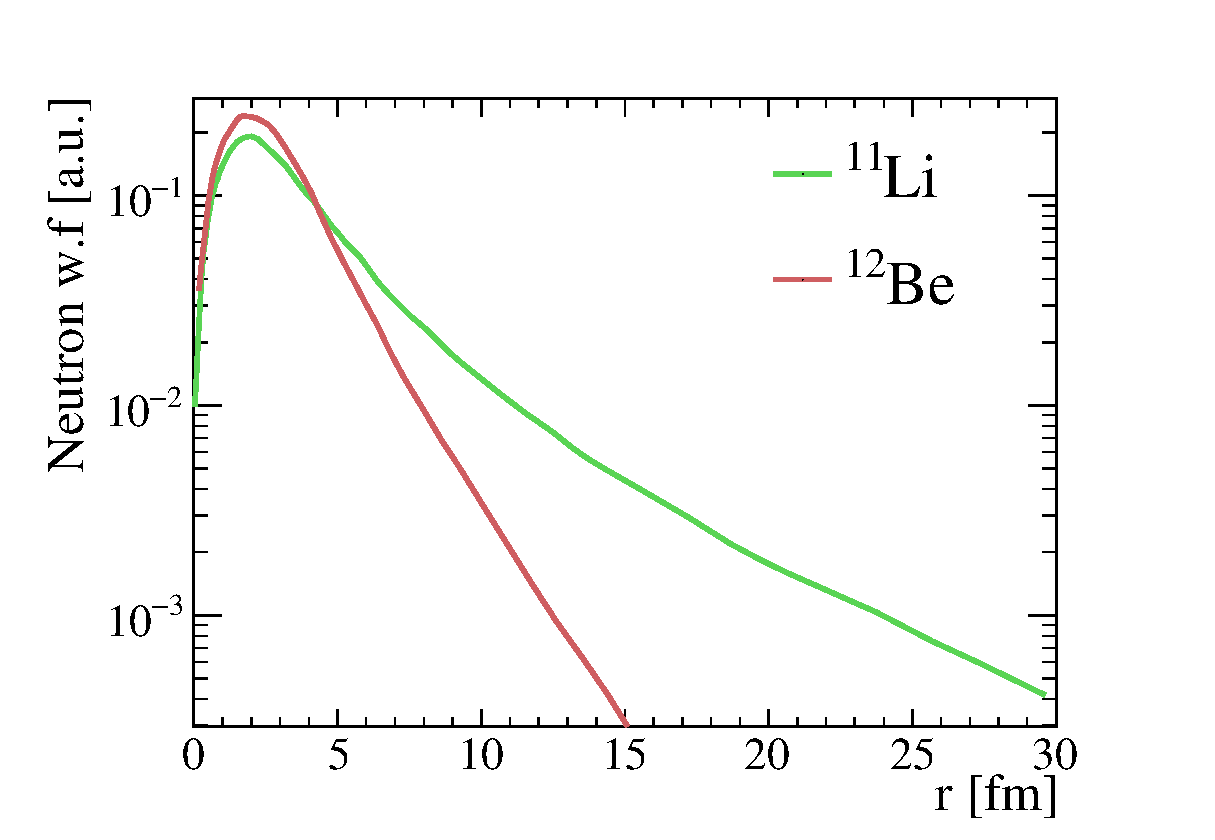
\includegraphics[width=1\linewidth]{figures/wfs.eps}};
                    \myscope[false]{
                        \draw[<->, very thick, dashed, magenta] (0.47, 0.25) -- (0.7, 0.25);
                    }
                \end{tikzpicture}
                \caption{N. K. Timofeyuk, private communication (in E748 proposal)}
            \end{figure}
        }
    \end{columns}
    \begin{columns}[c]
        \begin{column}{0.78\linewidth}
            \mycolorbox[1]{box4}{
                $\Rightarrow$ Need to establish more systematics for this parameter
            }
        \end{column}
    \end{columns}
    % \begin{column}{0.5\linewidth}
    %     \mycolorbox[0.95]{box4}{
    %         \begin{itemize}
    %             \item Measure $\left\langle\iso{10,12}{Be}\middle|\iso{9,11}{Li}\right\rangle$
    %             \item $\Delta S = -12.8 | -19.8 \unit{\MeV}$
    %         \end{itemize}
    %     }
    % \end{column}%
    % \begin{column}{0.5\linewidth}
    %     \mycolorbox{box1}{
    %         \begin{itemize}
    %             \item Establish systematics for \textbf{\color{magenta} GMF}
    %         \end{itemize}
    %     }
    % \end{column}
    % \end{columns}
\end{frame}

\begin{frame}{Physics case of E748}
    E748 @ GANIL back in 2017. Using \iso{10,12}{Be}(d,\iso{3}{He}) reactions to:
    \bigskip
    \begin{columns}[T]
        \begin{column}{0.52\linewidth}
            \mycolorbox[1]{box2}{
            Overlaps:
            {\small
            \begin{itemize}
                \item $\left\langle\iso{10}{Be}\middle|\iso{9}{Li}\right\rangle, \Delta S = \qty{-12.8}{\MeV}$
                \item $\left\langle\iso{12}{Be}\middle|\iso{11}{Li}\right\rangle, \Delta S = \textcolor{magenta}{\qty{-19.8}{\MeV}}$
            \end{itemize}}
            \begin{tikzpicture}
                \node[anchor=south west, inner sep = 0pt] (image) at(0, 0){
                    \includegraphics[width=0.6\linewidth]{figures/Be_proton_shell_model.pdf}
                };
                \myscope[false]{
                \node[pin={[pin distance=4mm, pin edge={<-, very thick, magenta}]-90:{\footnotesize This strength}}] at (0.75, 0.7) {};
                }
            \end{tikzpicture}
            }
        \end{column}
        \begin{column}{0.48\linewidth}
            \mycolorbox[1]{box3}{\small
                Explore effects of GMF:
                \begin{itemize}
                    \item $\left\langle\iso{10}{Be}\middle|\iso{9}{Li}\right\rangle, \text{GMF} \sim \num{1}$
                    \item $\left\langle\iso{12}{Be}\middle|\iso{11}{Li}\right\rangle, \text{GMF} \sim \textcolor{blue}{\num{0.5}?}$
                \end{itemize}
                \begin{tikzpicture}[
                        % background rectangle/.style={fill=white},
                        % show background rectangle,
                        trim left=-27,
                    ]
                    \centering
                    \begin{axis}[
                            width=0.63\linewidth,
                            scale only axis,
                            % xlabel={Potential},
                            ylabel={GMF},
                            % minor y tick num=1,
                            xticklabels={$\overlap{\iso{11}{Li}}{\iso{10}{He}}$,
                                    \textcolor{magenta}{$\overlap{\iso{10}{Be}}{\iso{9}{Li}}$},
                                    \textcolor{magenta}{$\overlap{\iso{12}{Be}}{\iso{11}{Li}}$}},
                            xtick={1,2,3},
                            xmin=0.75, xmax=3.25,
                            ymin=0, ymax=1,
                            ymajorgrids=true, yminorgrids=true,
                            ytick distance=0.25,
                            grid style = {dashed},
                            x tick label style = {font=\tiny},
                        ]
                        \addplot+ [
                            error bars/.cd,
                            y dir=both,y explicit,
                        ] coordinates {
                                (1, 0.25) +- (0,0)
                                (2, 1) +- (0,0)
                                (3, 0.65) +- (0, 0.15)
                            };
                    \end{axis}
                \end{tikzpicture}
                % \begin{tikzpicture}[scale=0.8]
                %     \datavisualization [
                %         scientific axes={inner ticks},
                %         visualize as line=gmf,
                %         gmf={style={mark=o}},
                %         x axis={length=0.8\linewidth, include value=0, include value=2,
                %                 ticks={major at={
                %                                 0 as $\overlap{\iso{11}{Li}}{\iso{10}{He}}$,
                %                                 1 as [style=magenta] $\overlap{\iso{10}{Be}}{\iso{9}{Li}}$,
                %                                 2 as [style=magenta] $\overlap{\iso{12}{Be}}{\iso{11}{Li}}$
                %                             }}},
                %         y axis={label={GMF}, include value=0, include value=1}]
                %     data [format=TeX code]{
                %             \pgfkeys{/data point/.cd,x=0, y=0.25} \pgfdatapoint
                %             \pgfkeys{/data point/.cd,x=1, y=1} \pgfdatapoint
                %             \pgfkeys{/data point/.cd,x=2, y=0.5} \pgfdatapoint
                %         };
                % \end{tikzpicture}
            }
        \end{column}
    \end{columns}
\end{frame}

\section{Methodology}
\begin{frame}[c]{Experimental setup}
    Tradional solid target experiment @ LISE
    \vspace{1.5em}
    \includegraphics[width=1\linewidth]{figures/setup.pdf}
\end{frame}

\begin{frame}[t]{A glance at the analysis}
    \begin{columns}[T]
        \begin{column}{0.48\linewidth}
            \mycolorbox{box4}{
                \enumitem{1} \textbf{Heavy} ID at \qty{0}{\degree}
            }
            \begin{tikzpicture}
                \node[anchor = south west, inner sep = 0pt] (image) at (0,0){
                    \includegraphics[width=1\linewidth]{figures/heavy.png}
                };
                \myscope[false]{
                \node[pin={
                [pin distance=5mm,
                        pin edge={<-, very thick, ForestGreen}]0:{Be}}
                ] at (0.60, 0.42) {};
                \node[pin={
                [pin distance=5mm,
                        pin edge={<-, very thick, color=ForestGreen}]0:{Li}}
                ] at (0.60, 0.28) {};
                }
            \end{tikzpicture}
        \end{column}
        \begin{column}{0.48\linewidth}
            \mycolorbox{box2}{
                \enumitem{2} \textbf{Light} PID in DSSD
            }
            \begin{tikzpicture}
                \node[anchor=south west, inner sep=0pt] (image) at(0,0){
                    \includegraphics[width=1\linewidth]{figures/light.png}
                };
                \myscope[false]{
                    \node[pin={[pin distance=16mm, pin edge={<-, line width = 1.5pt, orange}]-87:A = 1}] at (0.2, 0.65) {};
                    \node[pin={[pin distance = 10mm, pin edge={<-, line width=1.5pt, orange}]-80:A = 2}] at (0.25, 0.65) {};
                    \node[pin={[pin distance=8mm, pin edge={<-, line width=1.5pt, orange}]-70:A = 3}] at (0.4, 0.7) {};
                    \node[pin={[pin distance=4mm, pin edge={<-, line width = 1.5pt, orange}]-75:A = 4}] at (0.6, 0.72) {};
                }
            \end{tikzpicture}
        \end{column}
    \end{columns}
    \mycolorbox{box1}{
        \enumitem{3} $E_{x}$ from \textbf{missing mass technique}
        $E_{\textrm{beam}} + (E,\theta)_{\textrm{Lab}} \rightarrow E_{x}$
    }
\end{frame}

\section{Results}
\begin{frame}[t]{Results: \texorpdfstring{\iso{10}{Be}(d,\iso{3}{He})\iso{9}{Li} }{10Be(d,3He)9Li}}
    \only<+>{
        \begin{columns}[T]
            \begin{column}{0.5\linewidth}
                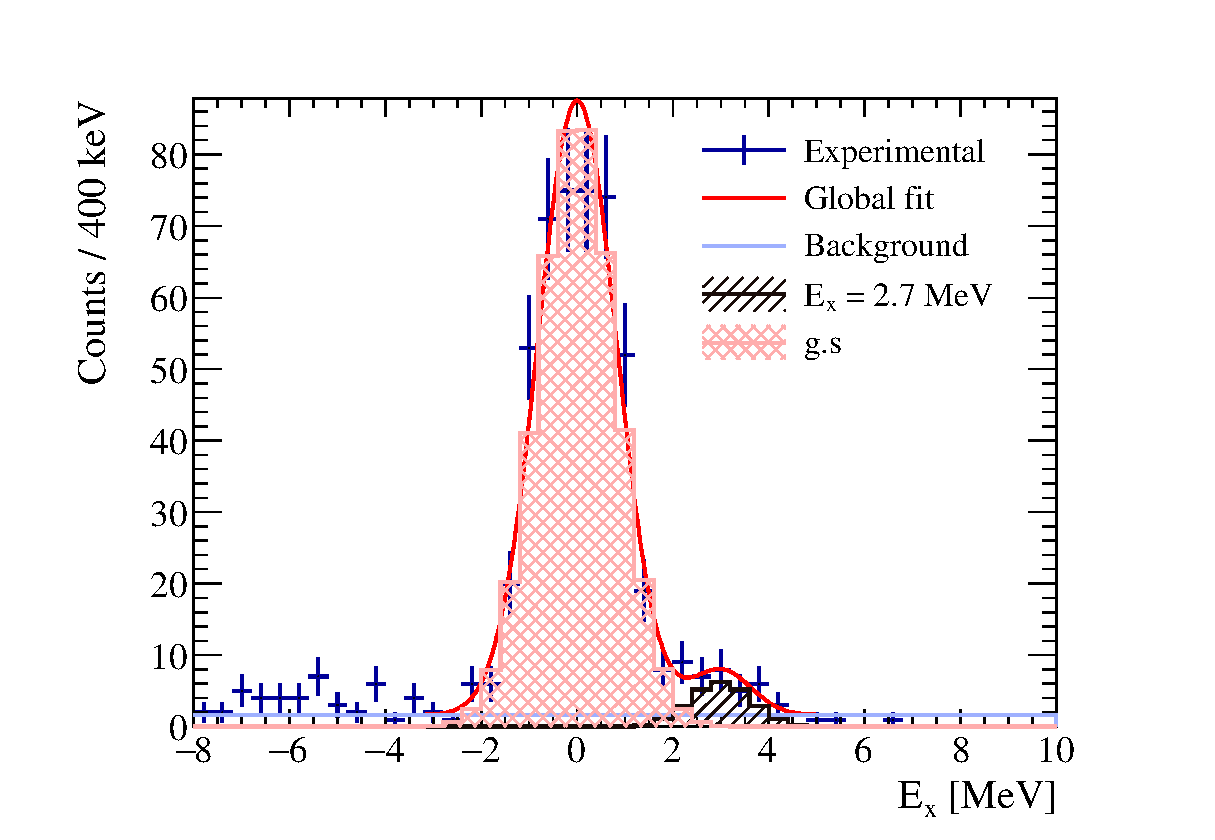
\includegraphics[width=\textwidth]{figures/10Be_d3He_fit.eps}
            \end{column}
            \begin{column}{0.5\linewidth}
                \includegraphics[width=\textwidth]{figures/10Be_d3He_xs.eps}
            \end{column}
        \end{columns}
    }
    \only<+>{
    The \textbf{first} excited state $1/2^{-}$ is also accessible.
    \begin{columns}[T]
        \begin{column}{0.5\linewidth}
            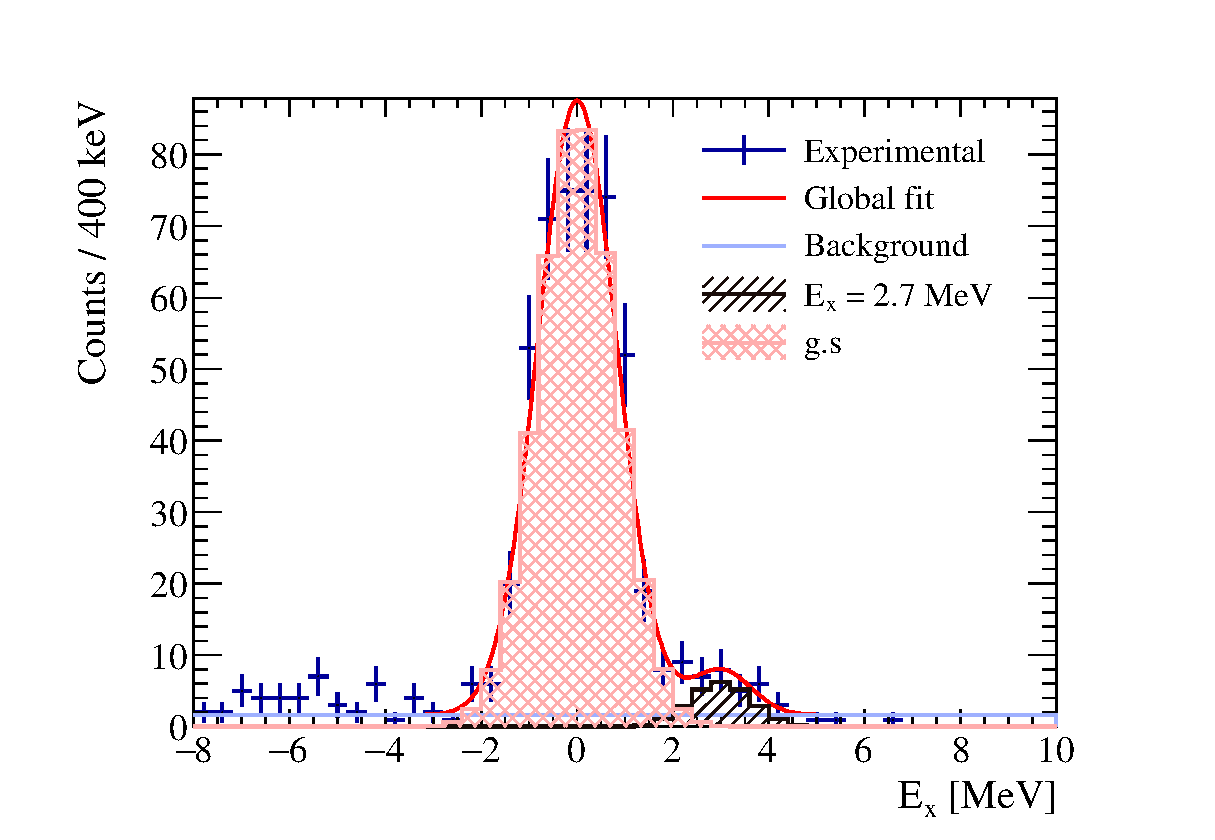
\includegraphics[width=\textwidth]{figures/10Be_d3He_fit.eps}
        \end{column}
        \begin{column}{0.5\linewidth}
            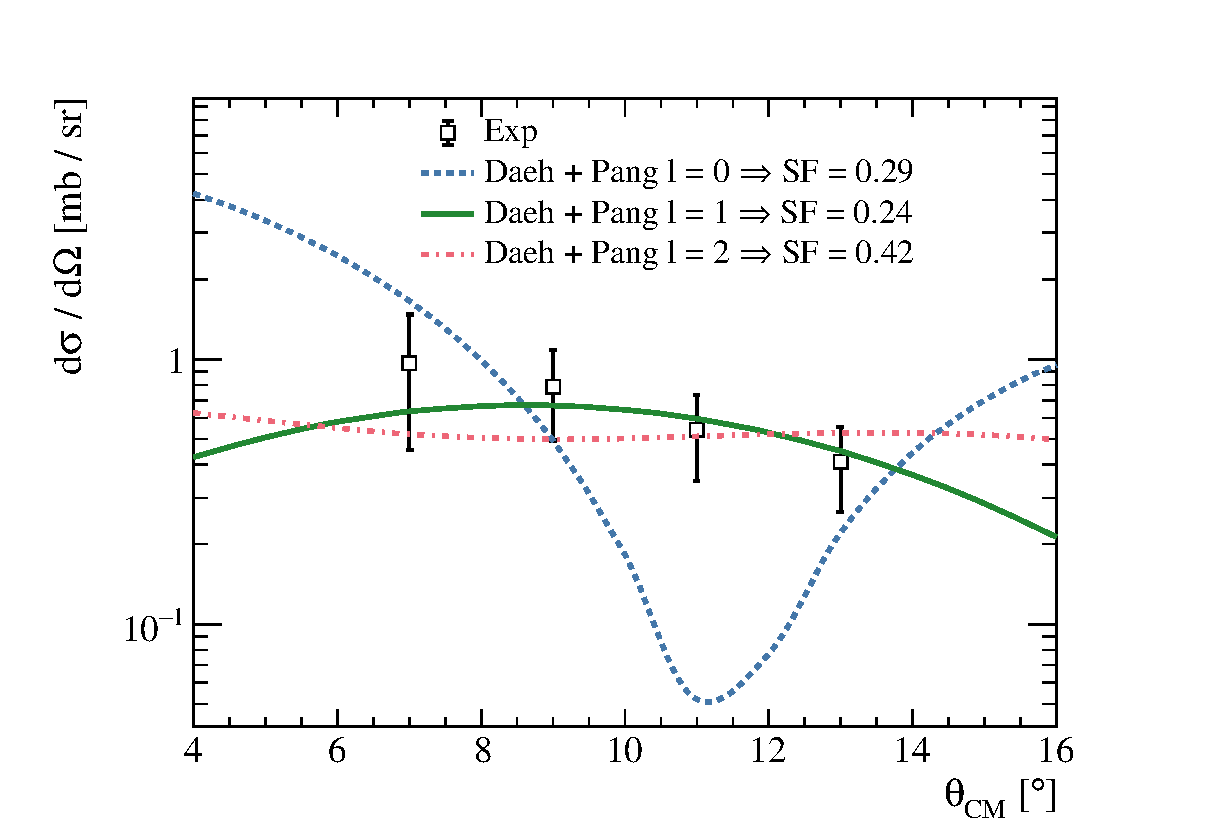
\includegraphics[width=\textwidth]{figures/10Be_d3He_xs_g1.eps}
        \end{column}
    \end{columns}
    \vspace{1.5em}
    \begin{columns}[c]
        \begin{column}{0.48\linewidth}
            \mycolorbox[1]{box2}{
                \textbf{First} direct measurement:\\
                $C^{2}S = \qty{0.237(46)}{}$
            }
        \end{column}
        \begin{column}{0.48\linewidth}
            \mycolorbox[1]{box1}{
                SM calculation by Acculina:\\
                $C^{2}S = \qty{0.207}{}$}
        \end{column}
    \end{columns}
    }
    \only<+>{
        \begin{columns}[T]
            \begin{column}{0.5\linewidth}
                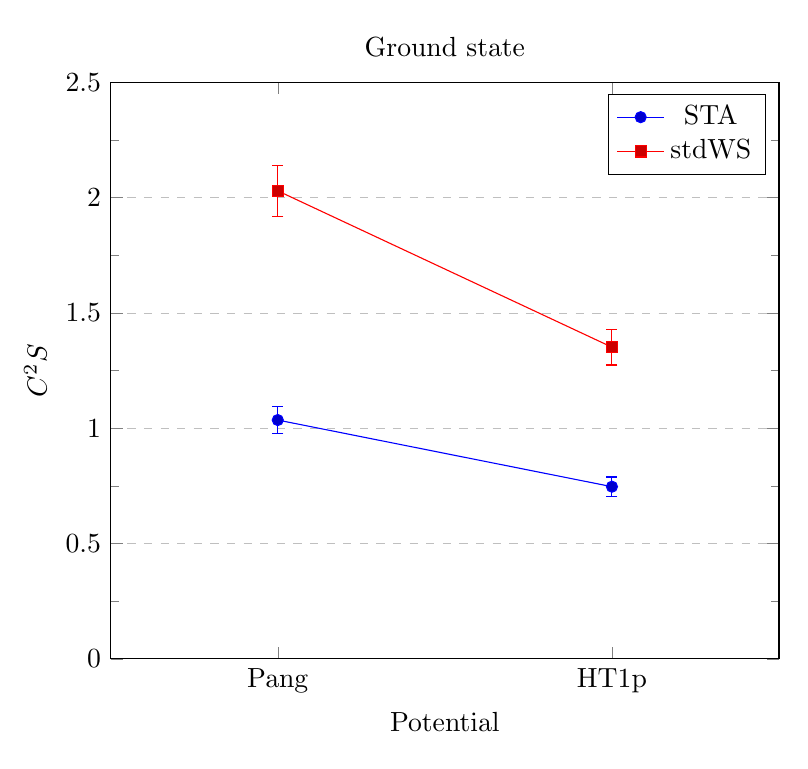
\begin{tikzpicture}[
                        % background rectangle/.style={fill=white},
                        % show background rectangle,
                        trim left=-30,
                    ]
                    \centering
                    \begin{axis}[
                            width=0.7\linewidth,
                            scale only axis,
                            title={Ground state},
                            xlabel={Potential},
                            ylabel={$C^{2}S$},
                            minor y tick num=1,
                            xticklabels={Pang, HT1p},
                            xtick={1,2},
                            xmin=0.5, xmax=2.5,
                            ymin=0, ymax=2.5,
                            ymajorgrids=true, yminorgrids=false,
                            ytick distance=0.5,
                            legend style={fill=none},
                            grid style = {dashed},
                        ]
                        \addplot+ [
                            error bars/.cd,
                            y dir=both,y explicit,
                        ] coordinates {
                                (1, 1.036) +- (0,0.058)
                                (2, 0.747) +- (0,0.042)
                            };
                        \addplot+ [
                            error bars/.cd,
                            y dir=both,y explicit,
                        ] coordinates {
                                (1, 2.03) +- (0,0.11)
                                (2, 1.352) +- (0,0.077)
                            };
                        \legend{STA, stdWS}
                    \end{axis}
                \end{tikzpicture}
            \end{column}
            \begin{column}{0.5\linewidth}
                \begin{tikzpicture}[
                        % background rectangle/.style={fill=white},
                        % show background rectangle,
                        trim left=-30,
                    ]
                    \centering
                    \begin{axis}[
                            width=0.7\linewidth,
                            scale only axis,
                            title={1st excited},
                            xlabel={Potential},
                            ylabel={$C^{2}S$},
                            minor y tick num=1,
                            xticklabels={Pang, HT1p},
                            xtick={1,2},
                            xmin=0.5, xmax=2.5,
                            ymin=0, ymax=0.5,
                            ymajorgrids=true, yminorgrids=false,
                            ytick distance=0.25,
                            legend style={fill=none},
                            grid style={dashed},
                        ]
                        \addplot+ [
                            error bars/.cd,
                            y dir=both,y explicit,
                        ] coordinates {
                                (1, 0.146) +- (0,0.028)
                                (2, 0.104) +- (0,0.020)
                            };
                        \addplot+ [
                            error bars/.cd,
                            y dir=both,y explicit,
                        ] coordinates {
                                (1, 0.054) +- (0,0.011)
                                (2, 0.219) +- (0,0.043)
                            };
                        \legend{STA, stdWS}
                    \end{axis}
                \end{tikzpicture}
            \end{column}
        \end{columns}
    }
\end{frame}

\begin{frame}[t]{Results: \texorpdfstring{\iso{12}{Be}(d,\iso{3}{He})\iso{11}{Li} }{12Be(d,3He)11Li}}
    \begin{columns}[T]
        \begin{column}{0.5\linewidth}
            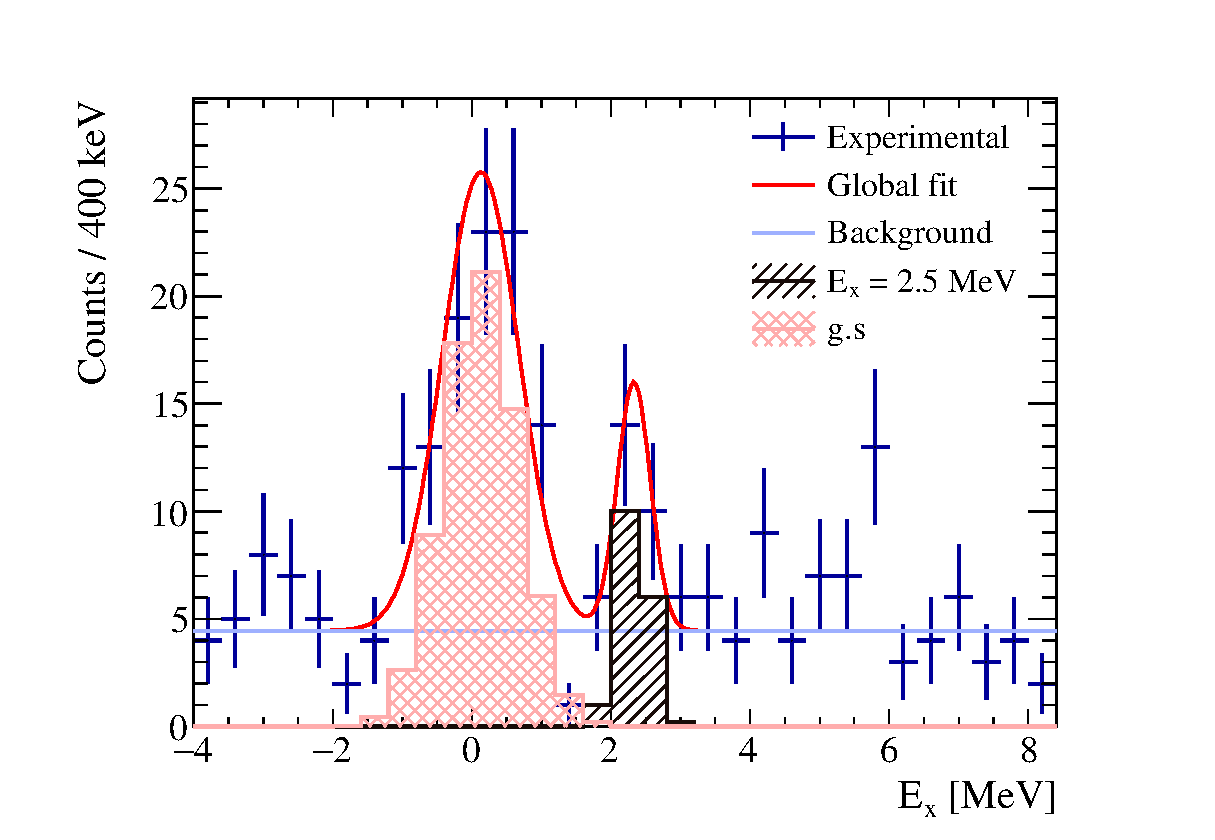
\includegraphics[width=\textwidth]{figures/12Be_d3He_fit.eps}
        \end{column}
        \begin{column}{0.5\linewidth}
            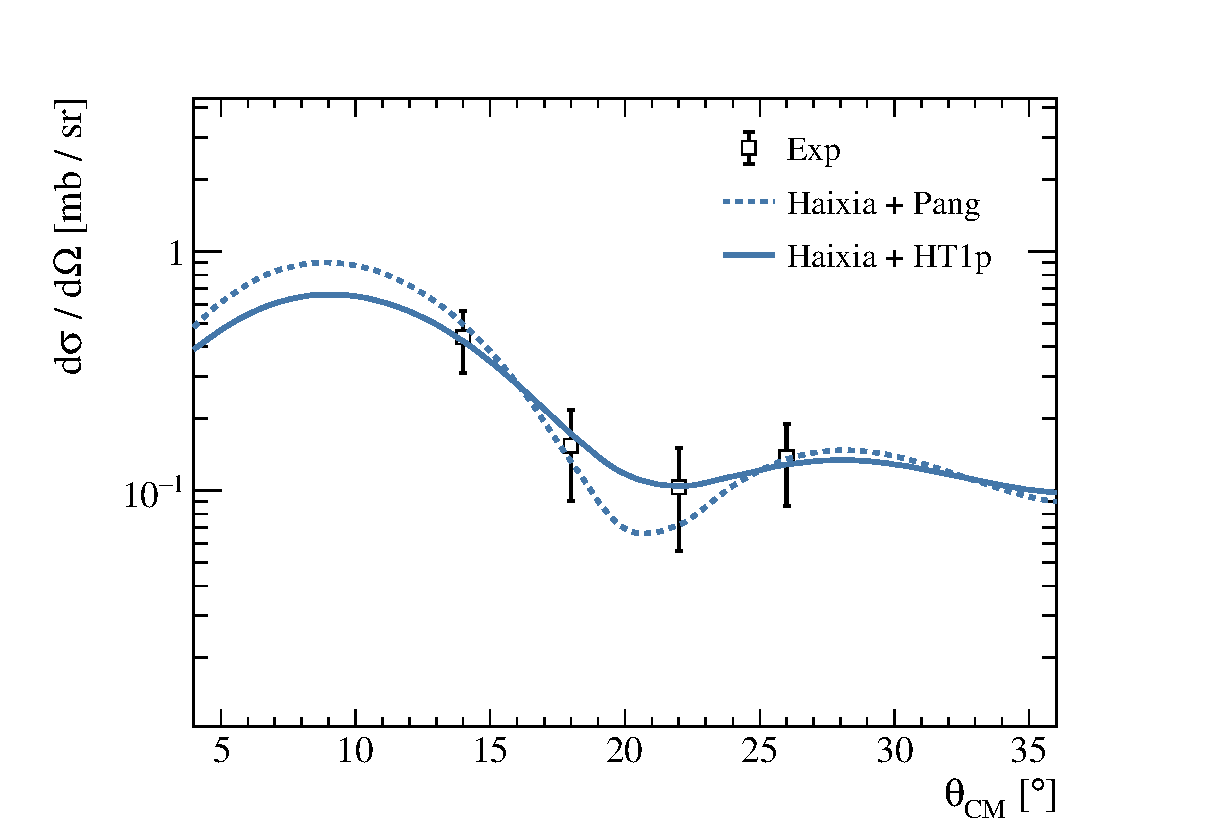
\includegraphics[width=\textwidth]{figures/12Be_d3He_xs.eps}
        \end{column}
    \end{columns}
    \begin{columns}[c]
        \begin{column}{0.48\linewidth}
            \mycolorbox[1]{box2}{
                \begin{enumerate}
                    \item $C^{2}S = \qty{0.33}{}$ with Haixia + HT1p
                    \item Need to solve puzzle with different OMPs
                \end{enumerate}}
        \end{column}
        \begin{column}{0.48\linewidth}
            \mycolorbox[1]{box3}{
                Fulfils expectation of:\\
                $0.65 (\text{quenching}) \cdot 0.5 (\text{GMF})$\\
                This is true with Pang but not with HT1p...
            }
        \end{column}
    \end{columns}
\end{frame}

\begin{frame}[t]{Conclusions}
    The reduction factor $\text{R}_{\text{S}}$ is computed using SM $C^{2}S$ from the SFO-tls interaction.
    \begin{figure}
        \centering
        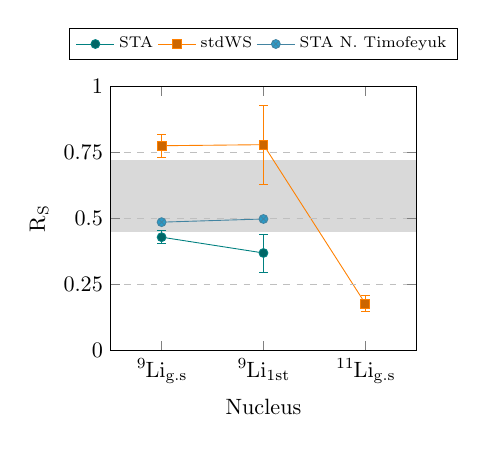
\begin{tikzpicture}[
                % background rectangle/.style={fill=white},
                % show background rectangle,
                trim left=-30,
                scale=0.8,
            ]
            \begin{axis}[
                width=0.4\linewidth,
                scale only axis,
                xlabel={Nucleus},
                ylabel={$\text{R}_{\text{S}}$},
                % minor y tick num=1,
                xticklabels={$\iso{9}{Li}_{\text{g.s}}$, $\iso{9}{Li}_{\text{1st}}$, $\iso{11}{Li}_{\text{g.s}}$},
                xtick={1,2,3},
                xmin=0.5, xmax=3.5,
                ymin=0, ymax=1,
                ymajorgrids=true, yminorgrids=false,
                ytick distance=0.25,
                legend style={
                        fill=none,
                        anchor=south,
                        at={(0.5, 1.1)},
                        font=\scriptsize,
                    },
                legend columns=3,
                grid style={dashed},
                axis on top,
                cycle list name=exotic,
                ]
                \addplot[fill=black!15, draw=none, forget plot] coordinates {(\pgfkeysvalueof{/pgfplots/xmin}, 0.45) (\pgfkeysvalueof{/pgfplots/xmax}, 0.45)  (\pgfkeysvalueof{/pgfplots/xmax}, 0.72) (\pgfkeysvalueof{/pgfplots/xmin}, 0.72)};
                \addplot+ [
                    error bars/.cd,
                    y dir=both,y explicit,
                ] coordinates {
                        (1, 0.429) +- (0, 0.024)
                        (2, 0.369) +- (0, 0.072)
                    };
                \addplot+ [
                    error bars/.cd,
                    y dir=both,y explicit,
                ] coordinates {
                        (1, 0.776) +- (0, 0.044)
                        (2, 0.78) +- (0, 0.15)
                        (3, 0.177) +- (0, 0.030)
                    };
                \addplot+ [
                    error bars/.cd,
                    y dir=both,y explicit,
                ] coordinates {
                        (1, 0.486) +- (0, 0)
                        (2, 0.498) +- (0, 0)
                    };
                \legend{STA, stdWS, STA N. Timofeyuk}
            \end{axis}
        \end{tikzpicture}
    \end{figure}
    And now what?
\end{frame}

\begin{frame}[plain]{Acknowledgments}
    \begin{columns}[T]
        \begin{column}{0.33\linewidth}
            The E748 collaboration:
            \begin{itemize}\scriptsize
                \item Santiago:\\
                      B. Fernández
                \item LPC-Caen:\\
                      A. Matta\\
                      F. Delaunay\\
                      N. L. Achouri\\
                      F. Flavigny\\
                      J. Gibelin\\
                      M. Marques\\
                      N. Orr
                \item IJCLab:\\
                      D. Beaumel\\
                      M. Assié\\
                      Y. Blumenfeld\\
                      S. Franchoo\\
                      A. Georgiadou\\
                      V. Girard-Alcindor\\
                      F. Hammache\\
                      N. de Séreville\\
                      A. Meyer\\
                      I. Stefan
            \end{itemize}
        \end{column}
        \begin{column}{0.33\linewidth}
            \begin{itemize}\scriptsize
                \item GANIL:\\
                      B. Jacquot\\
                      O. Kamalou\\
                      A. Lemasson\\
                      M. Rejmund\\
                      T. Roger\\
                      O. Sorlin\\
                      J.C. Thomas\\
                      M. Vandebrouck\\
                      B. Bastin\\
                      F. de Oliveira\\
                      C. Stodel
                \item RIKEN:\\
                      S. Koyama\\
                      D. Suzuki
                \item Surrey:\\
                      N. Timofeyuk
            \end{itemize}

        \end{column}
        \begin{column}{0.33\linewidth}
            \includegraphics[width=0.6\linewidth]{logos/usc_blue.png}\vspace{1em}
            \includegraphics[width=0.6\linewidth]{logos/lpc.png}\vspace{1em}
            \includegraphics[width=0.6\linewidth]{logos/ganil.png}\vspace{1em}
            \includegraphics[width=0.6\linewidth]{logos/ijclab.png}\vspace{1em}
            \includegraphics[width=0.6\linewidth]{logos/riken.png}\vspace{1em}
            \includegraphics[width=0.6\linewidth]{logos/surrey.png}\vspace{1em}
        \end{column}
    \end{columns}
\end{frame}

\begin{frame}[noframenumbering, plain]
    \begin{tikzpicture}[remember picture, overlay]
        \node at (current page.center) {
            \usebeamerfont{frame title}
            \textcolor{mainBlue}{Backup}
        };
    \end{tikzpicture}
\end{frame}

\begin{frame}[noframenumbering]{Elastic cross sections}
    Normalization of all cross-sections was obtained from fits to the elastic data using the Haixa potential.
    \begin{columns}[T]
        \begin{column}{0.5\linewidth}
            \begin{tikzpicture}
                \node[anchor=south west, inner sep=0pt] (image) at(0, 0){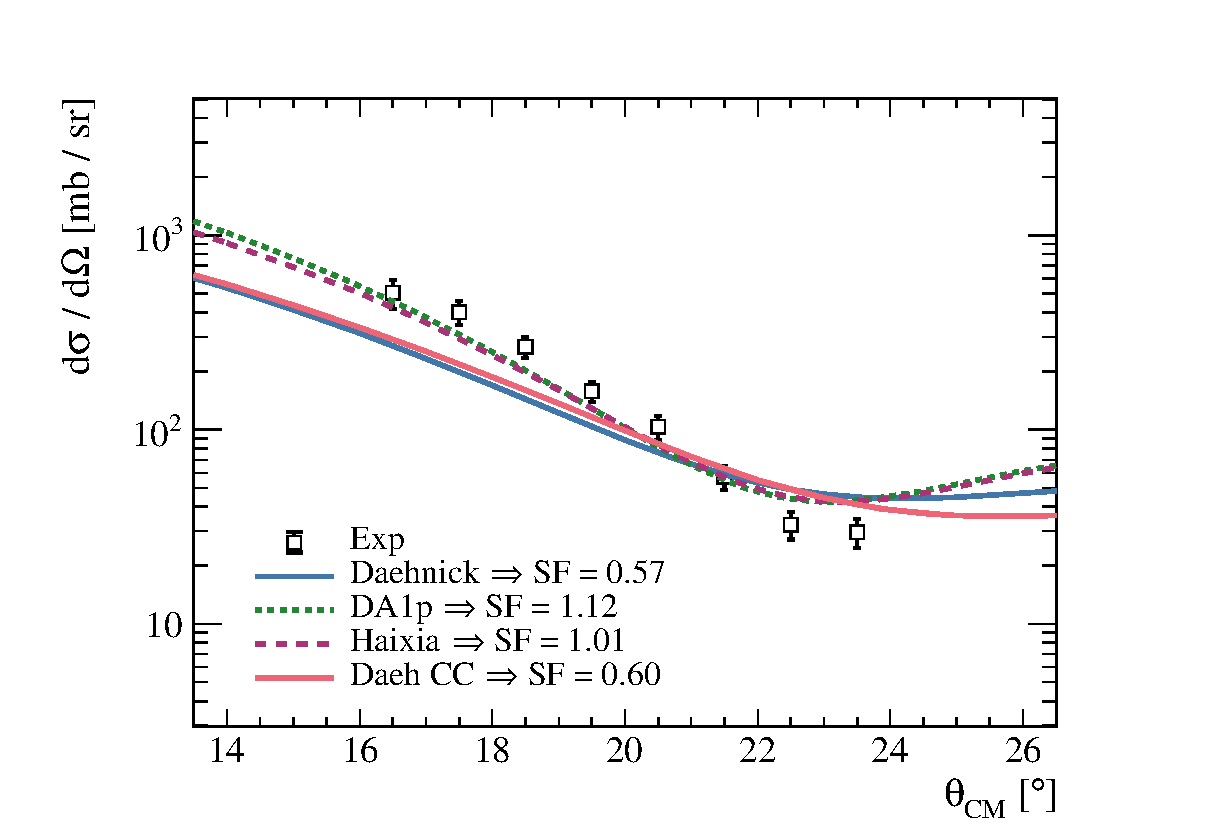
\includegraphics[width=1\linewidth]{figures/10Be_dd_xs.eps}};
                \myscope[false]{
                    \node at (image.north) {\iso{10}{Be}(d,d)};
                }
            \end{tikzpicture}
        \end{column}
        \begin{column}{0.5\linewidth}
            \begin{tikzpicture}
                \node[anchor=south west, inner sep=0pt] (image) at(0, 0){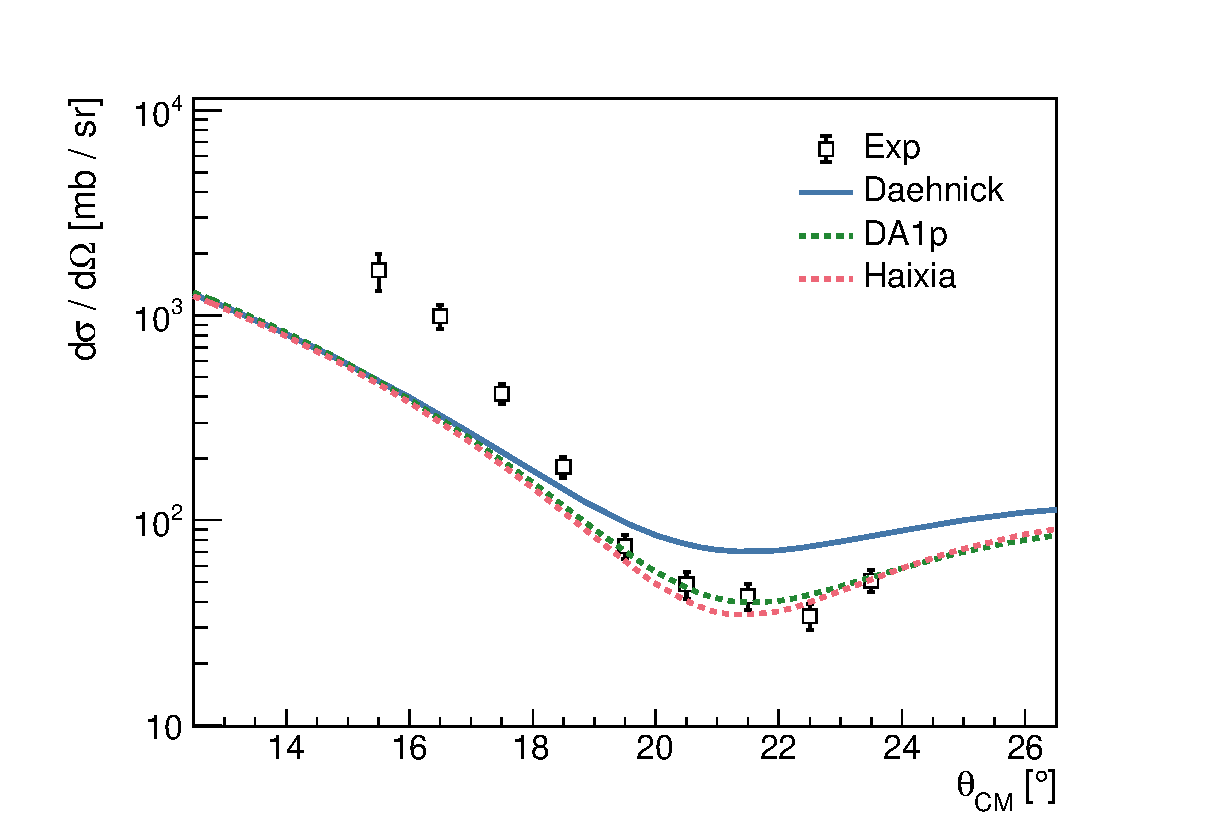
\includegraphics[width=1\linewidth]{figures/12Be_dd_xs.eps}};
                \myscope[false]{
                    \node at (image.north) {\iso{12}{Be}(d,d)};
                }
            \end{tikzpicture}
        \end{column}
    \end{columns}
    \vspace{1.25em}
    \mycolorbox{box2}{
        Best OMP: new ones DA1p and Haixia!
    }
\end{frame}

\begin{frame}[noframenumbering]{Crosscheck: \texorpdfstring{\iso{10}{Be}(d,t)\iso{9}{Be} }{10Be(d,t)9Be}}
    \begin{columns}[T]
        \begin{column}{0.5\linewidth}
            \only<1>{
                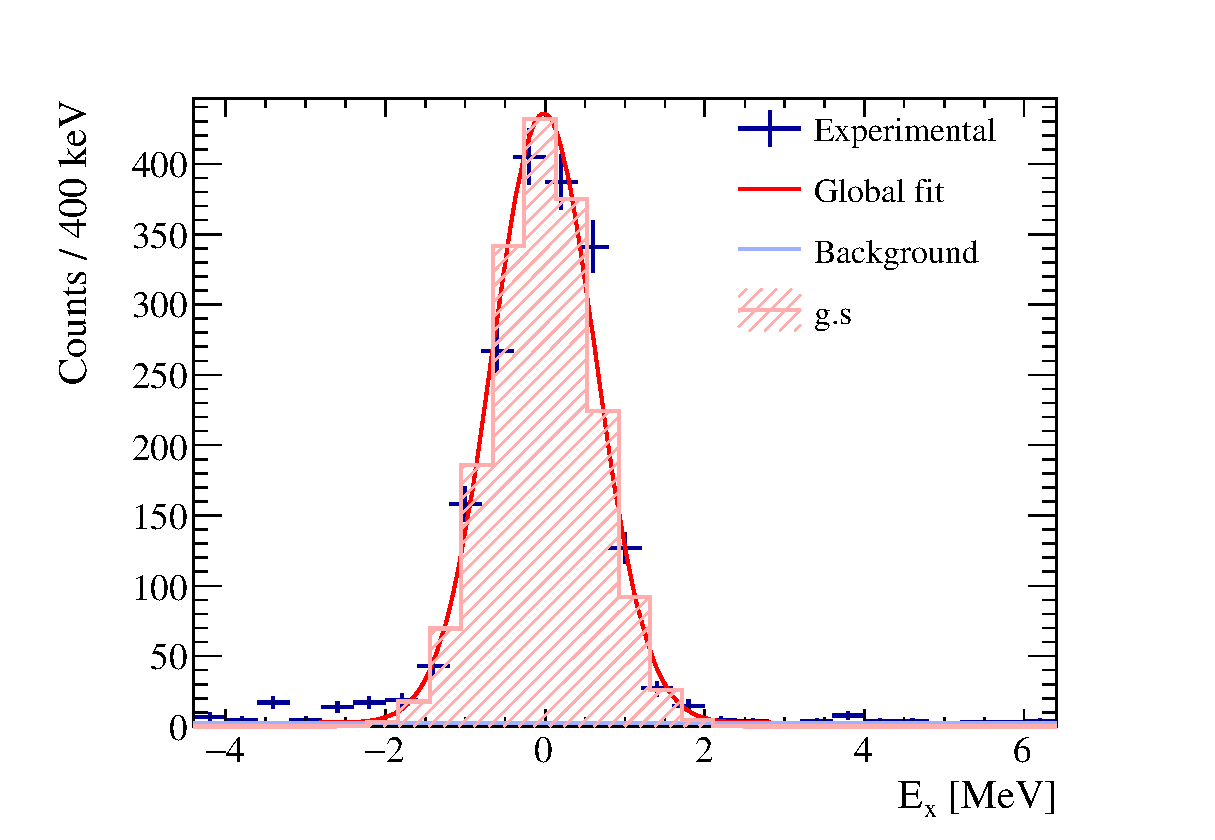
\includegraphics[width=\textwidth]{figures/10Be_dt_fit.eps}
            }
            \only<2>{
                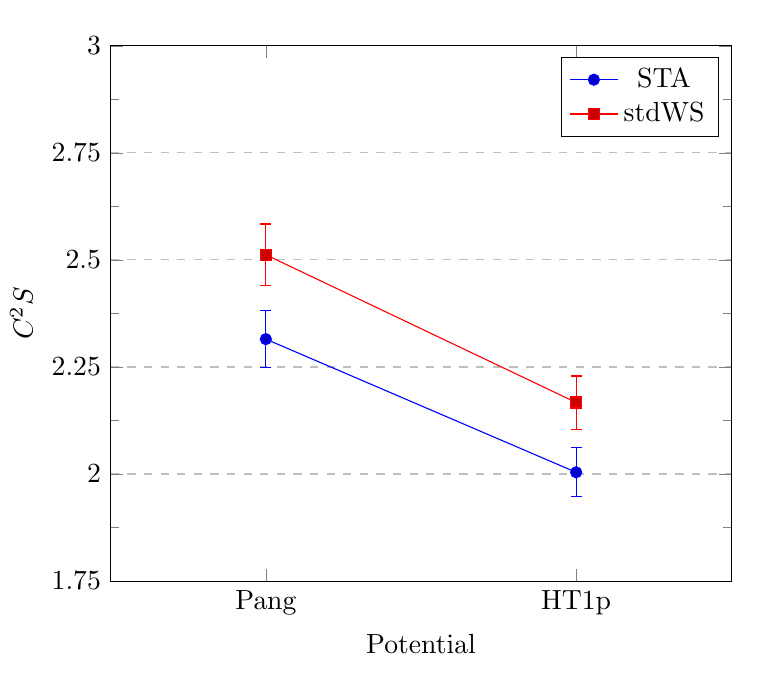
\begin{tikzpicture}[
                        % background rectangle/.style={fill=white},
                        % show background rectangle,
                        trim left=-30,
                    ]
                    \centering
                    \begin{axis}[
                            width=0.65\linewidth,
                            scale only axis,
                            % title={},
                            xlabel={Potential},
                            ylabel={$C^{2}S$},
                            minor y tick num=1,
                            xticklabels={Pang, HT1p},
                            xtick={1,2},
                            xmin=0.5, xmax=2.5,
                            ymin=1.75, ymax=3,
                            ymajorgrids=true, yminorgrids=false,
                            ytick distance=0.25,
                            legend style={fill=none},
                            grid style={dashed},
                        ]
                        \addplot+ [
                            error bars/.cd,
                            y dir=both,y explicit,
                        ] coordinates {
                                (1, 2.315) +- (0,0.066)
                                (2, 2.004) +- (0,0.057)
                            };
                        \addplot+ [
                            error bars/.cd,
                            y dir=both,y explicit,
                        ] coordinates {
                                (1, 2.512) +- (0,0.072)
                                (2, 2.167) +- (0,0.062)
                            };
                        \legend{STA, stdWS}
                    \end{axis}
                \end{tikzpicture}
            }
        \end{column}
        \begin{column}{0.5\linewidth}
            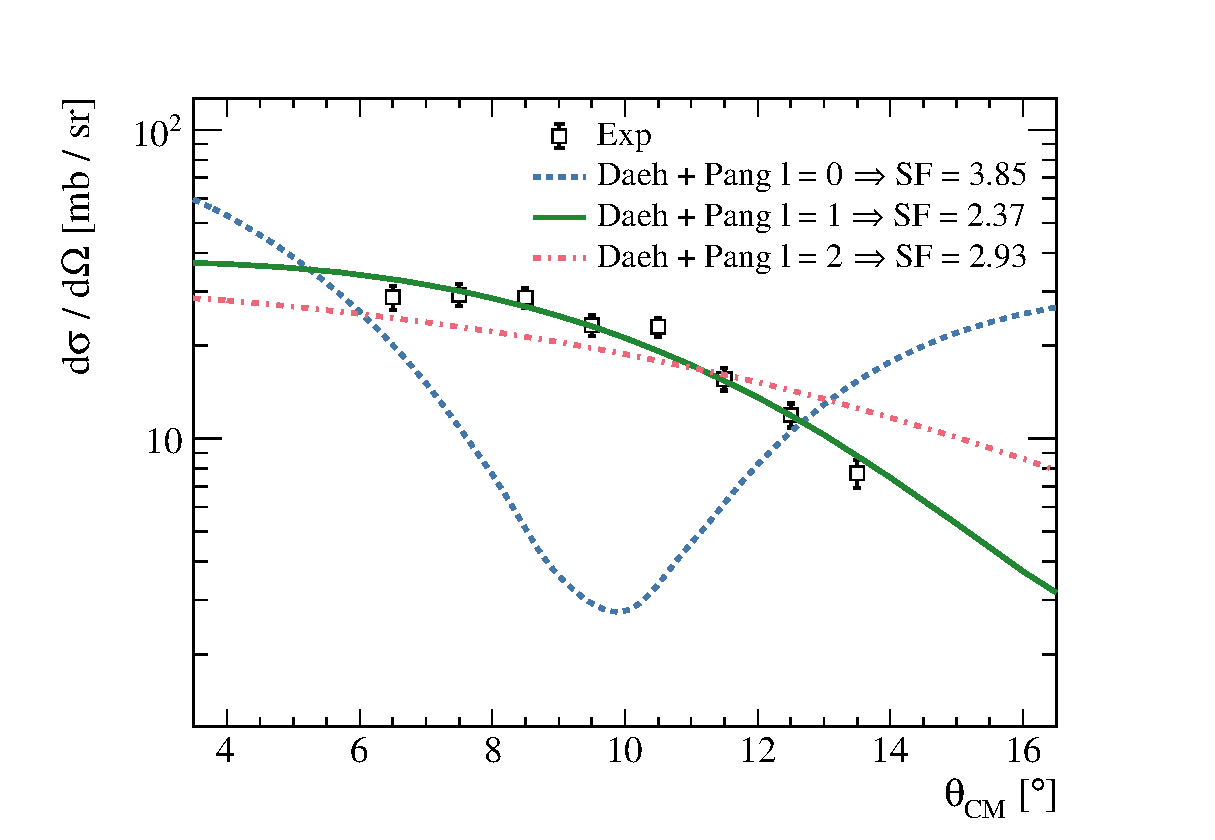
\includegraphics[width=\textwidth]{figures/10Be_dt_xs.eps}
        \end{column}
    \end{columns}
    \vspace{1.5em}
    \begin{columns}[c]
        \begin{column}{0.48\linewidth}
            \mycolorbox[1]{box2}{
                \textbf{Best fit} is a $\ell = 1$\\
                $C^{2}S = \qty{2.370(69)}{}$
            }
        \end{column}
        \begin{column}{0.48\linewidth}
            \mycolorbox[1]{box4}{
                In accordance with $\sim \qty{60}{\percent}$ quenching of SFs
            }
        \end{column}
    \end{columns}
\end{frame}

\begin{frame}[noframenumbering]{Kinematical lines}
    \begin{columns}[T]
        \begin{column}{0.5\linewidth}
            \begin{tikzpicture}
                \node[anchor=south west, inner sep=0pt] (image) at(0, 0){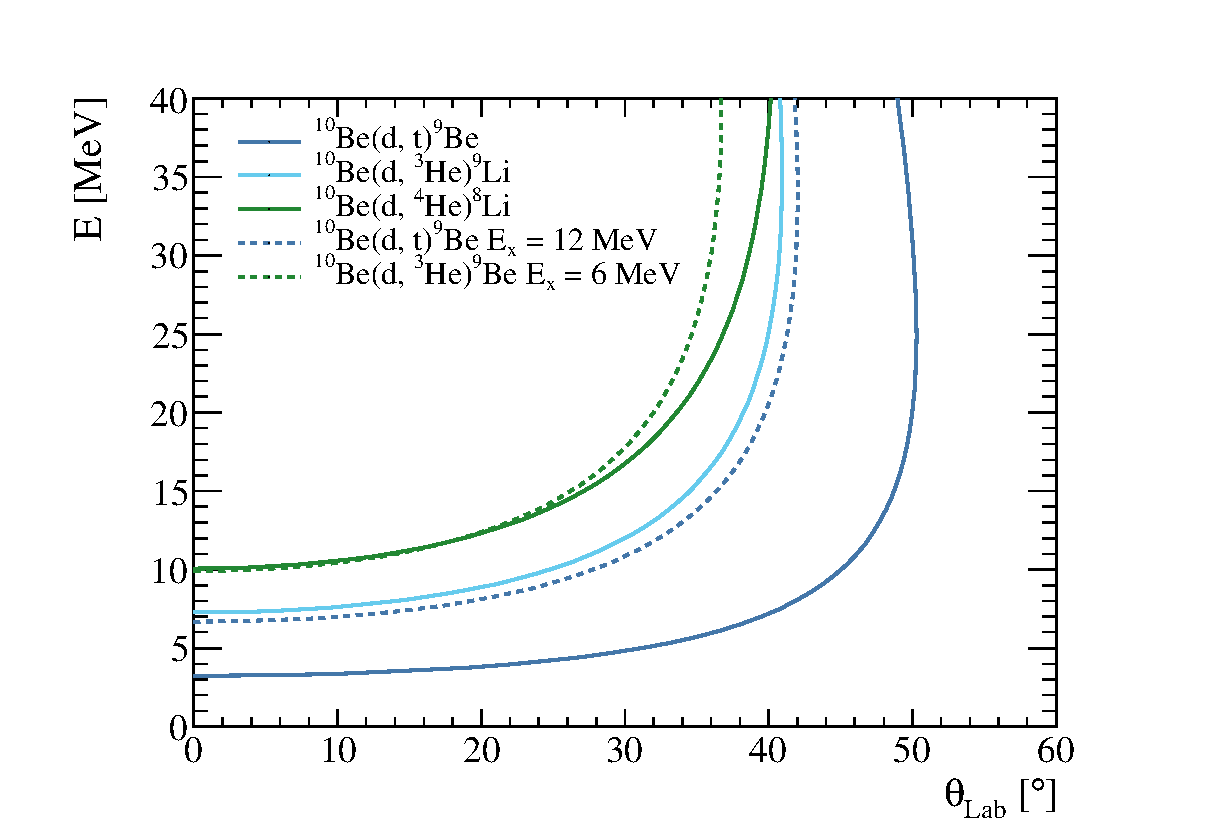
\includegraphics[width=1\linewidth]{figures/kin_10Be.eps}};
                \myscope[false]{
                    \node at (image.north) {\iso{10}{Be}};
                }
            \end{tikzpicture}
        \end{column}
        \begin{column}{0.5\linewidth}
            \begin{tikzpicture}
                \node[anchor=south west, inner sep=0pt] (image) at(0, 0){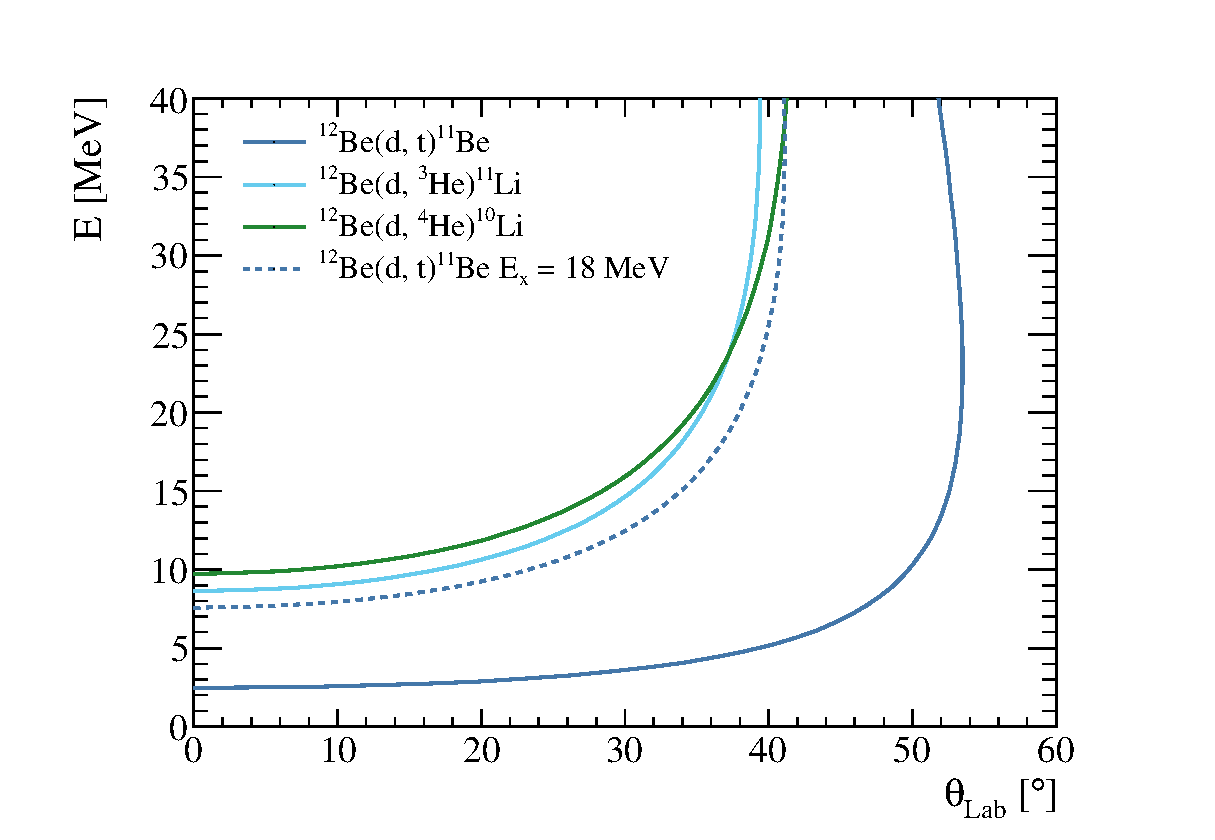
\includegraphics[width=1\linewidth]{figures/kin_12Be.eps}};
                \myscope[false]{
                    \node at (image.north) {\iso{12}{Be}};
                }
            \end{tikzpicture}
        \end{column}
    \end{columns}
\end{frame}

\end{document}